\documentclass[14pt,aspectratio=169]{beamer}
\setbeamertemplate{caption}[numbered]
\setbeamertemplate{caption label separator}{:}
\setbeamercolor{caption name}{fg=normal text.fg}
\usepackage{amssymb,amsmath}
\usepackage{ifxetex,ifluatex}
\usepackage{fixltx2e} % provides \textsubscript
\usepackage{lmodern}
\ifxetex
  \usepackage{fontspec,xltxtra,xunicode}
  \defaultfontfeatures{Mapping=tex-text,Scale=MatchLowercase}
  \newcommand{\euro}{€}
\else
  \ifluatex
    \usepackage{fontspec}
    \defaultfontfeatures{Mapping=tex-text,Scale=MatchLowercase}
    \newcommand{\euro}{€}
  \else
    \usepackage[T1]{fontenc}
    \usepackage[utf8]{inputenc}
      \fi
\fi
% use upquote if available, for straight quotes in verbatim environments
\IfFileExists{upquote.sty}{\usepackage{upquote}}{}
% use microtype if available
\IfFileExists{microtype.sty}{\usepackage{microtype}}{}
\PassOptionsToPackage{hyphens}{url}
\usepackage{hyperref}
\usepackage{ulem}

% Comment these out if you don't want a slide with just the
% part/section/subsection/subsubsection title:
\AtBeginPart{
  \let\insertpartnumber\relax
  \let\partname\relax
  \frame{\partpage}
}
\AtBeginSection{
  \let\insertsectionnumber\relax
  \let\sectionname\relax
  \begin{frame}[plain]
    \tableofcontents[currentsection]
  \end{frame}
}
\AtBeginSubsection{
  \let\insertsubsectionnumber\relax
  \let\subsectionname\relax
  \frame{\subsectionpage}
}

\setlength{\parindent}{0pt}
\setlength{\parskip}{6pt plus 2pt minus 1pt}
\setlength{\emergencystretch}{3em}  % prevent overfull lines
\setcounter{secnumdepth}{0}
% Thanks Richard Darst on how to get a nice Beamer theme.
% See http://rkd.zgib.net/wiki/DebianBeamerThemes

\usepackage{multicol}
\usepackage{tikz}
\usepackage{ctable}
\usetikzlibrary{positioning}

\usebackgroundtemplate{
\includegraphics[width=\paperwidth]{images/swirl-lightest.pdf}}
\logo{
\includegraphics[viewport=274 335 360 440,width=1cm]{images/openlogo-nd.pdf}}

\definecolor{debianred}{rgb}{.780,.000,.211} % 199,0,54
\definecolor{debianblue}{rgb}{0,.208,.780} % 0,53,199
\definecolor{debianlightbackgroundblue}{rgb}{.941,.941,.957} % 240,240,244
\definecolor{debianbackgroundblue}{rgb}{.776,.784,.878} % 198,200,224

\usetheme{Boadilla}
\setbeamertemplate{navigation symbols}{}

\usecolortheme[named=debianbackgroundblue]{structure}
\setbeamercolor{normal text}{fg=black}
\setbeamercolor{titlelike}{fg=debianblue}
\setbeamercolor{sidebar}{fg=debianred,bg=debianbackgroundblue}

\setbeamercolor{palette sidebar primary}{fg=debianred}
\setbeamercolor{palette sidebar secondary}{fg=debianred}
\setbeamercolor{palette sidebar tertiary}{fg=debianred}
\setbeamercolor{palette sidebar quaternary}{fg=debianred}

\setbeamercolor{section in toc}{fg=debianred}
\setbeamercolor{subsection in toc}{parent=debianred}

\setbeamercolor{item}{fg=debianred}

\setbeamercolor{block title}{fg=debianblue}

\title[Reproducible Builds]{Reproducible Builds: \\ The original promise of free software}

\author[lamby]{%
   \texorpdfstring{
            \centering
            Chris Lamb \\ 
            \href{mailto:lamby@debian.org}{lamby@debian.org}
   }{lamby}}
\date[skroutz.gr '15]{%
 skroutz.gr (Athens, Greece)
}

\begin{document}

\begin{frame}
\titlepage
\end{frame}

\section{About}

\begin{frame}[fragile]
 \frametitle{The problem}
 \begin{itemize}
  \item Original promise of free software \pause
  \item Anyone can view source code \pause
  \item But distributions provide compiled packages \pause
  \item Can we trust this process?
 \end{itemize}
\end{frame}

\begin{frame}[fragile]
 \pause
 \begin{itemize}
  \item Incentives to crack developer machines \pause
  \item \texttt{CVE-2002-0083}: remote root exploit in OpenSSH - single bit difference in binary \pause
  \item Trojaned Apple SDK \pause
  \item Rootkit modifying the source code in memory only
 \end{itemize}
\end{frame}

\begin{frame}
 \begin{center}
  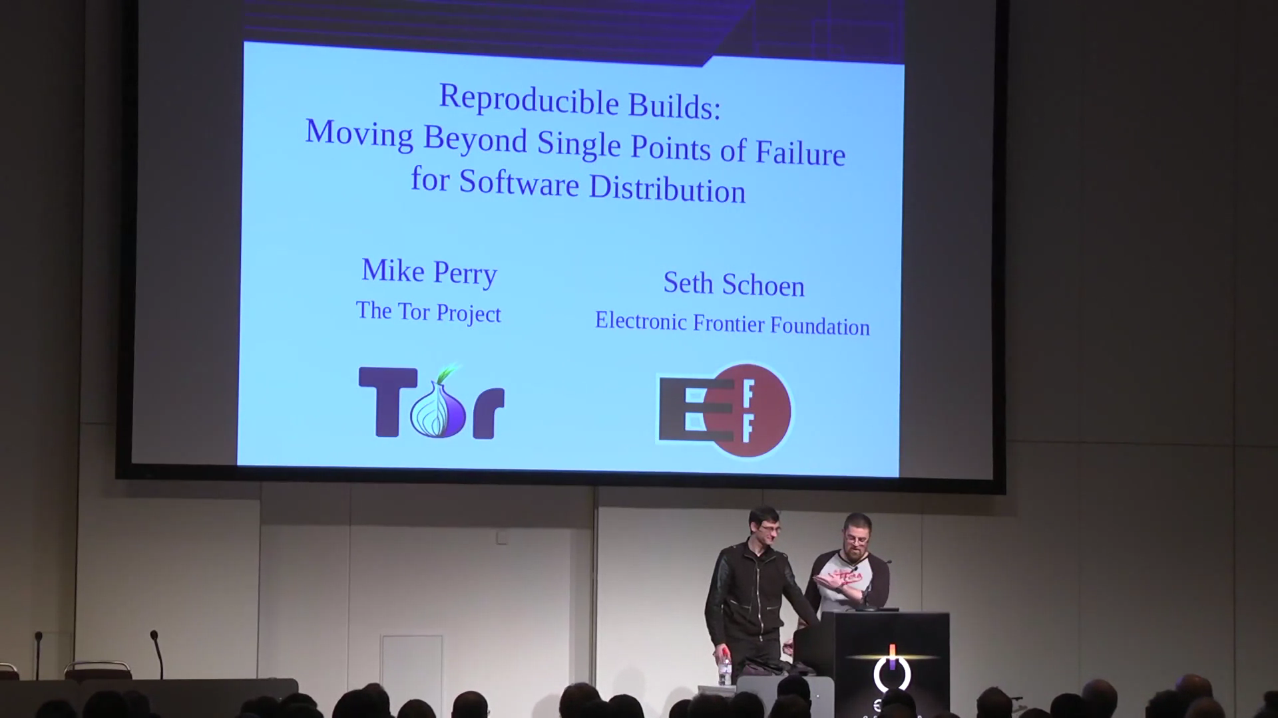
\includegraphics[width=0.7\textwidth]{images/31c3.png}
  \\
  Available on \url{media.ccc.de}, 31c3
 \end{center}
\end{frame}

\begin{frame}[fragile]
 CIA conference in 2012:
 \begin{center}
  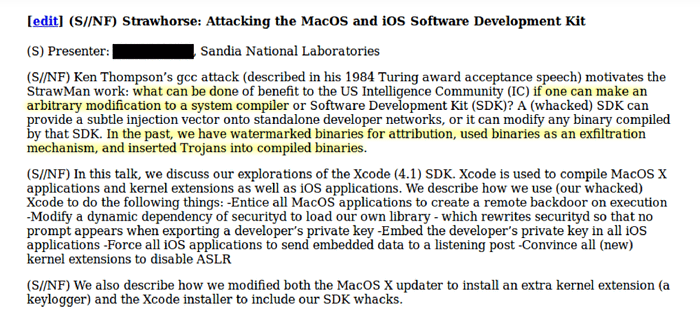
\includegraphics[width=0.8\textwidth]{images/strawhorse.png}

  {\footnotesize
  \url{firstlook.org/theintercept/2015/03/10/ispy-cia-campaign-steal-apples-secrets/}
  }
 \end{center}
\end{frame}

\begin{frame}[fragile]
 \frametitle{The solution} \pause
 \begin{itemize}
  \item Ensure that compilation always produces the same result \pause
  \item Bit-for-bit identical \pause
  \item Multiple parties compare signatures \pause
  \item Attacker needs to infect all developers simultaneously \pause
  \item Can now trust what is running on your computers
 \end{itemize}

\end{frame}
\begin{frame}[fragile]
 \frametitle{Technical advantages} \pause
 \begin{itemize}
  \item Unsafe/unreliable behaviour (eg. internet access)
  \item Non-deterministic behaviour
  \item Being able to "go back in time"
  \item Detect corrupted build environments
  \item Easier to test changes/revisions
 \end{itemize}
\end{frame}


\section{Current progress}

\begin{frame}[fragile]
 \frametitle{Current projects} \pause
 \begin{itemize}
  \item Limited to Tor, Bitcoin, etc. \pause
  \item Really need an entire operating system
 \end{itemize}
\end{frame}

\begin{frame}[plain]
 \frametitle{Progress in Debian}
 \pause
 \begin{center}
  \includegraphics[height=0.73\paperheight]{images/stats_pkg_state.png}

  \footnotesize{19,257 out of 23,141 packages are reproducible}
  \vfill
 \end{center}
\end{frame}

\begin{frame}
 \frametitle{reproducible.debian.net}
 \pause

 \begin{itemize}
  \item Continuously testing \texttt{testing}, \texttt{unstable} and \texttt{experimental}
  \item Also testing coreboot, OpenWrt, NetBSD, FreeBSD and Archlinux.
 \end{itemize}
 \vfill
 \begin{center}
  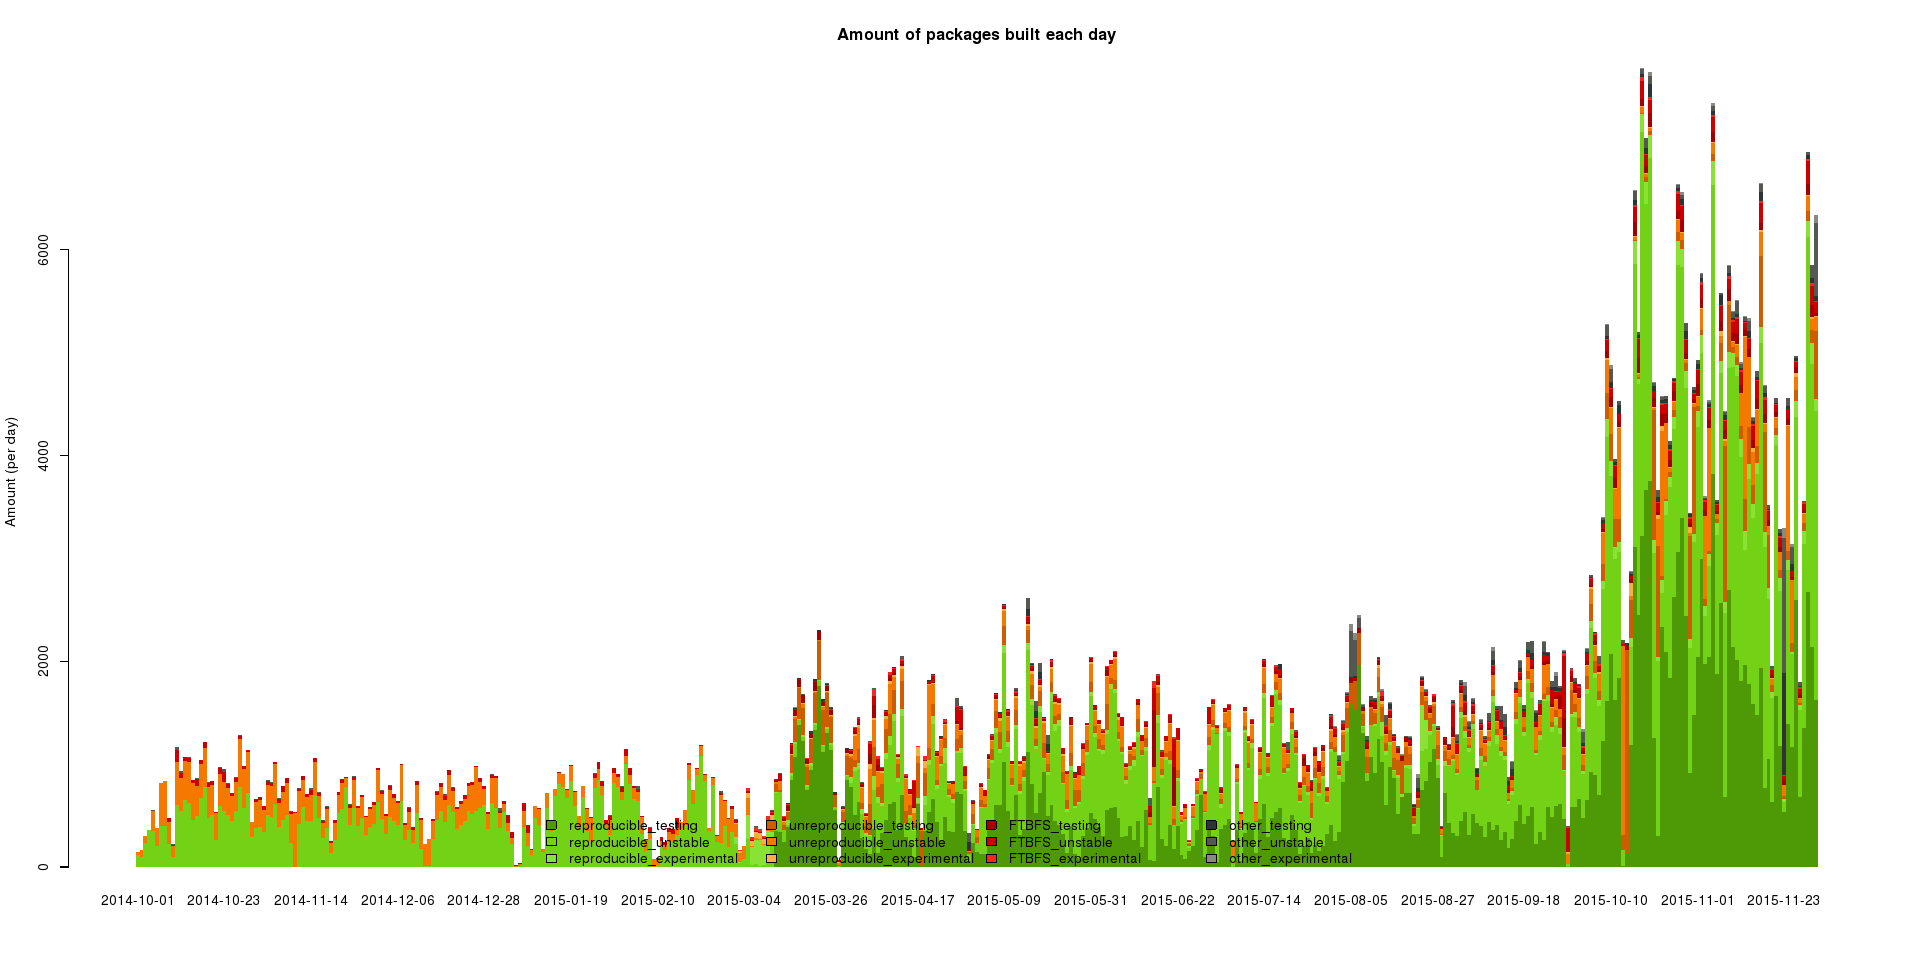
\includegraphics[height=0.47\paperheight]{images/stats_builds_per_day_amd64.png}
 \end{center}
\end{frame}

\begin{frame}[fragile]
 \frametitle{Variations}
 \pause

 \begin{center}
  \begin{table}
   \resizebox{0.95\textwidth}{!}{%
    \begin{tabular}{l|ll}
\textbf{variation} & \textbf{first build} & \textbf{second build} \\
\hline
hostname & \texttt{jenkins} & \texttt{i-capture-the-hostname} \\
domainname & \texttt{debian.net} & \texttt{i-capture-the-domainname} \\
\texttt{env TZ} & \texttt{GMT+12} & \texttt{GMT-14} \\
\texttt{env LANG} & \texttt{C} & \texttt{fr\_CH.UTF-8} \\
\texttt{env LC\_ALL} & not set & \texttt{fr\_CH.UTF-8} \\
\texttt{env USER} & \texttt{pbuilder1} & \texttt{pbuilder2} \\
uid & \texttt{1111} & \texttt{2222} \\
gid & \texttt{1111} & \texttt{2222} \\
UTS namespace & shared with the host & \textit{modified using \texttt{/usr/bin/unshare --uts}} \\
kernel version & Linux 3.16.0-4 / 4.2.0-0.bpo & Linux 2.6.56-4 / 2.6.62-0.bpo.1 \\
umask & 0022 & 0002 \\
CPU type & \multicolumn{2}{l}{same for both builds \textit{(work in progress)}} \\
filesystem & \multicolumn{2}{l}{same for both builds \textit{(work in progress - disorderfs)}} \\
year, month, date & \multicolumn{2}{l}{same for both builds \textit{(work in progress)}} \\
hour, minute & \multicolumn{2}{l}{hour is usually the same… usually, the minute differs… \textit{(work in progress)}} \\
\textit{everything else} & \multicolumn{2}{l}{\textit{is likely the same…}}
    \end{tabular}
   }
  \end{table}
 \end{center}
\end{frame}

\begin{frame}
 \frametitle{reproducible.debian.net}
 \begin{itemize}
  \item 12 hosts
  \item \texttt{amd64}: 111 cores and 198 GB RAM split between 9 VMs
  \item \texttt{armhf}: 18 cores and 9 GB RAM split between 6 systems
 \end{itemize}
 \begin{center}
  
\includegraphics[height=0.2\paperheight]{images/profitbricks_logo.png}
  \vfill
 \end{center}
\end{frame}


\begin{frame}
 \frametitle{Publicity}
 \begin{itemize}
  \item Summit in December 2015 (Athens)
   \begin{itemize}
    \item 40 people from 16 projects
   \end{itemize}
  \item Recent talks (some available with subtitles):
   \begin{itemize}
    \item 2015-08-13: Chaos Communication Camp 2015
    \item 2015-08-20: DebConf15
    \item 2015-11-08: Mini-DebConf Cambridge 2015
   \end{itemize}
  \item Weekly reports since May 2015
  \item LWN articles
  \item Lots of press
 \end{itemize}
\end{frame}

{
\usebackgroundtemplate{%
 \begin{tikzpicture}[remember picture,overlay]%
  \node[shift={(-0.15\paperwidth, 0.4\paperheight)},at=(current page.south east)] {
    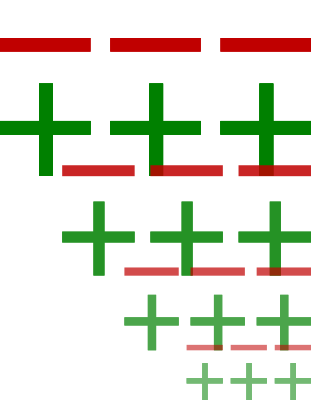
\includegraphics[width=0.2\paperwidth]{images/diffoscope_logo.png}
  };
 \end{tikzpicture}%
}
\begin{frame}{diffoscope}
 \frametitle{diffoscope}
 \begin{itemize}
  \item Examines differences \textbf{recursively}
  \item Outputs HTML / text with human readable differences
  \item Supports archives, uncompresses PDFs, disassembles binaries, unpacks Gettext files, etc.
  \item Binary comparison fallback
  \item Available from \texttt{git}, PyPI, Debian, Archlinux, Guix, Homebrew
  \item \url{http://diffoscope.org/}
 \end{itemize}
\end{frame}
}

\begin{frame}
 \begin{tikzpicture}[remember picture]
  \node[at=(current page.center)] {
   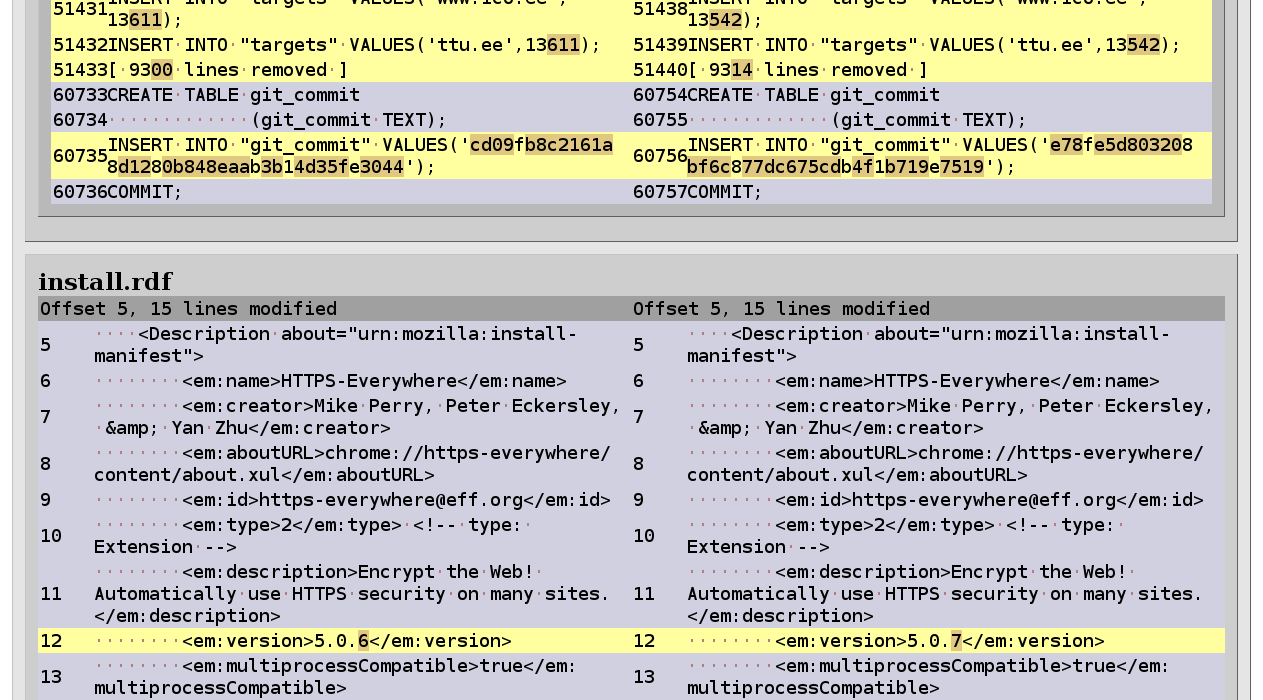
\includegraphics[width=0.9\paperwidth]{images/diffoscope_example_html.png}
  };
 \end{tikzpicture}
\end{frame}

\section{Get involved}

\begin{frame}
 \frametitle{As a developer} \pause
 \begin{itemize}
  \item Build something twice, run diffoscope on the result \pause
  \item Stop using build dates: \texttt{SOURCE\_DATE\_EPOCH}
 \end{itemize}
\end{frame}

\begin{frame}
 \frametitle{Join the team} \pause

 \begin{itemize}
   \item Individual issues \pause
   \item Toolchain issues \pause
   \item Tools: \texttt{reproducible.d.n}, diffoscope, etc. \pause
   \item Write documentation and talk to the world
 \end{itemize}
\end{frame}

\begin{frame}
 \pause
 \begin{center}
  \textbf{@lambyuk}
  \vskip 1em
  \texttt{https://chris-lamb.co.uk}
 \end{center}

 \vfill
  
 \begin{center}
  \resizebox{0.8\textwidth}{!}{%
   \begin{tabular}{rl}
    \texttt{lamby@debian.org} & \texttt{C2FE 4BD2 71C1 39B8 6C53} \\
                              & \texttt{3E46 1E95 3E27 D431 1E58}
   \end{tabular}
  }
 \end{center}
\end{frame}

\end{document}
